\section{Model}
\label{sec:model}

\subsection{Distribution network}

In this section, we present the model we used to solve the problem of ANM in DSO grid.
In particular, we will show how this problem can be cast as a MDP and how RL can be included when the distribution of the uncertainty is unknown and we will highlight the modeling assumptions used.

The electrical network can be mathematically modeled as a graph whose edges represent the electrical lines and whose nodes are locations in the network where power can be consumed or injected.
In a typical distribution network, the nodes correspond to households or small factories that behave as prosumers.
In this work, we will make the assumption that the graph is a tree as it is the case of most distribution networks.
Let $\mathcal{N}$ be the set of nodes and $\mathcal{E}$ be the set of edges.
Let $\mathcal{G}$ be the graph representing the network, i.e. $\mathcal{G} = (\mathcal{N}, \mathcal{E})$.

We represent every node by an integer in $\{0, \dots, n\}$ where $n = |\mathcal{N}|-1$ is the cardinality of set $\mathcal{N}$.
The root of the tree is the node that connects the distribution network to the transmission network and is the node $0$ in our model and we denote by $\mathcal{N}_+ = \mathcal{N} \backslash \{0\}$.
Each node $i \in \mathcal{N}_+$ has a unique ancestor denoted by $A_i$ and each node $i \in \mathcal{N}$ has a set of children denoted by $\mathcal{C}_i$.
We choose the orientation of the lines from being from $i$ to $A_i$ so that we can unambiguously represent each line by its origin node.
We thus have $\mathcal{E} = \{1, \dots, n\}$.
We will define the following nodal and branch quantities :

For each node $i \in \mathcal{N}$, we define :
\begin{itemize}
  \item $v_i$ as the square of the norm of the complex voltage at that node,
  \item $s_i = p_i + \mathbf{i} q_i$ as complex net power injection (the net injection being the power consumed minus the power produced)
  \item $d_i$ is the active net power injection demanded at node $i$, i.e. the power that the agent at that node wants to reinject in the network.
  It is thus different than the power that will actually be seen by the network (that is, $p_{i}$) as some curtailment mechanisms can take place.
  This will be further discussed later.
  It is positive when the power is injected and negative if it is retrieved.
\end{itemize}

For each line $i \in \mathcal{E}$, we define :
\begin{itemize}
  \item $z_i = r_i + \mathbf{i}x_i$ as the complex impedance,
  \item $l_i$ as the square of the norm of the complex current,
  \item $S_i = P_i + \mathbf{i}Q_i$ as the sending-end complex power, where $P_i$ denote the active power and $Q_i$ the reactive power.
\end{itemize}

A schematic representation of a line together with the notations we use is given in Figure~\ref{fig:line}.

\begin{figure}
  \begin{center}
    \begin{tikzpicture}[scale=8]
        \draw [->] (0,0.7) -- (0,0.53);
        \draw [->] (0.8,0.7) -- (0.8,0.53);
        \draw [thick] (0,0.5) -- (0.8, 0.5);
        \draw [<-] (0.25, 0.45) -- (0.55, 0.45);
        \node [left] at (0,0.7) {$s_{A_i}$};
        \node [right] at (0.8,0.7) {$s_i$};
        \node [below, left] at (0,0.5) {$v_{A_i}$};
        \node [below, right] at (0.8,0.5) {$v_i$};
        \node [above] at (0.4, 0.5) {$z_i$};
        \node [below] at (0.3, 0.45) {$l_i$};
        \node [below] at (0.5, 0.45) {$S_i$};
    \end{tikzpicture}
  \caption{Schematic representation of a line.}
  \label{fig:line}
  \end{center}
\end{figure}

We consider the problem in a multi-time-step framework.
This means that the variables are defined at each time step.
We consider a horizon of $T$ time steps.
The set of time steps is denoted by $\mathcal{T}$ and each one is represented by a positive integer, i.e. $\mathcal{T} = \{1, \dots, T\}$.

Moreover, we consider the context of a distribution system with a high level of renewable energy production.
We consider that each house has a PV installation and that the overproduction is reinjected in the network.
Therefore, the net power injection at each node can be decomposed into a power produced $p_{i,t}^p$ and a power consumed $p_{i,t}^c$ such that

\[ p_{i,t} = p_{i,t}^p - p_{i,t}^c \]

\subsection{Power flow equations}

For a radial distribution network, the equations that link all nodal and branch electrical quantities by taking \emph{Kirchhoff}'s laws into account are called the \emph{Power Flow equations}.
They can be written as~\cite{Farivar_Relax1}

\begin{align}
  & 0  =  p_{0,t} + \sum_{j\in \mathcal{C}_0} \Big(P_{j,t}-r_{j}l_{j,t} \Big), \hspace{0.5cm} \forall{t} \in \mathcal{T} \label{ACOPF1}\\
  & 0   =  q_{0,t} + \sum_{j\in \mathcal{C}_0} \Big( Q_{j,t}-x_{j}l_{j,t} \Big), \hspace{0.5cm} \forall{t} \in \mathcal{T} \label{ACOPF2}\\
  & v_{\mathcal{A}_i,t}  =   v_{i,t} -2(r_iP_{i,t} + x_iQ_{i,t}) + (r_i^2 + x_i^2)l_{i,t}, \\
  & \hspace{0.5cm} \forall i \in \mathcal{N}_{+}, \hspace{0.2cm} \forall{t} \in \mathcal{T} \label{ACOPF3}\\
  & P_{i,t} =  p_{i,t} + \sum_{j\in \mathcal{C}_i} \Big( P_{j,t}-r_{j}l_{j,t} \Big), \hspace{0.5cm} \forall i \in \mathcal{N}_{+}, \hspace{0.2cm} \forall{t} \in \mathcal{T} \label{ACOPF4}\\
  & Q_{i,t}  =  q_{i,t} + \sum_{j\in \mathcal{C}_i} \Big( Q_{j,t}-x_{j}l_{j,t} \Big), \hspace{0.5cm} \forall i \in \mathcal{N}_{+}, \hspace{0.2cm} \forall{t} \in \mathcal{T} \label{ACOPF5}\\
  & v_{i,t}l_{i,t} = P_{i,t}^2 + Q_{i,t}^2, \hspace{0.5cm} \forall i \in \mathcal{N}_{+}, \hspace{0.2cm} \forall{t} \in \mathcal{T} \label{ACOPF:quad}
\end{align}

With these equations, the power injection at each node is sufficient to obtain the values of all other electrical quantities.

\subsection{Uncertainty}

These power injection, however, is subject to uncertainty.
They depend on the consumption and the production at each node.
We consider that forecast values, denoted by $\tilde{p}_{i,t}^p$ and $\tilde{p}_{i,t}^c$ are available to the DSO and the uncertainty can thus be modeled as the deviation from these forecast values.
Let us denote by $\delta_t^p$ and $\delta_t^c$ the deviation for, respectively, the production and the consumption at time step $t$.
These deviations are common to all nodes.
This is motivated by the fact that this uncertainty usually relies to external factor as solar irradiance, temperature, etc.
When the uncertain deviations are known, the power injections can be written as
\[
   p_{i,t}^p = \tilde{p}_{i,t}^p + \delta_t^p\tilde{p}_{i,t}^p
  \]
and
\[
   p_{i,t}^c = \tilde{p}_{i,t}^c + \delta_t^c\tilde{p}_{i,t}^c
  \]
We consider the following discrete sample space $\mathcal{P}$ for both type of deviation :
\[
  \mathcal{P} = \{0.1, 0, -0.1\}
\]
with an unknown probability distribution.
This means that we suppose that both the consumption and the production can either be $10\%$ more than the forecast value, exactly the forecast value or $-10\%$ of the forecast value.

\subsection{Flexible loads}
In modern distribution networks, some loads are more flexible than others.
Flexible loads can include small factories who sign contracts with the DSO allowing it to disconnect the factory from the network for some time.
In this work, we consider that there is a set $\mathcal{F}$ of flexible loads.
They are either in the state \emph{on} or \emph{off}.
For these loads, we consider that there are no production but only consumption.

\subsection{Set of states}

The state of the system is made of the time step in which we are, the level of the deviation from the forecast values for both the consumption and the production and the state of the flexible loads.
The state is represented by a vector of length $2+|\mathcal{F}|$ where the two first elements correspond to the deviation from respectively the production and the consumption and the $|\mathcal{F}|$ last elements are the binay states of the flexible loads ($0$ or $1$).
We denote by $\mathcal{S}$ the set of states and by $\mathcal{S}_t$ the set of states for a fixed $t$.
We have that
\begin{align*}
  \mathcal{S}_t = \{&(0.1, 0.1, 0, \dots, 0), (0, 0.1,0, \dots, 0), \dots, \\
                    &(-0.1, -0.1,1, \dots, 1)\} \\
\end{align*}
Note that $|\mathcal{S}_t| = 3^2 2^{|\mathcal{F}|} = 9 \cdot 2^{|\mathcal{F}|}$ and that $\mathcal{S}_t$ is independent of $t$.

\subsection{Control actions}

We consider that the action the DSO has to control its network is the curtailment of all or part of the PV production at each node and the choice of activating or not each flexible load, all of these at each time step.
By curtailing excessive solar production, the reliability of the network could be greatly increased.
This curtailment is also expressed as a percentage of the total injection seen by the network.
We denote by $\overline{p}_{i,t}$ the curtailment decided for node $i \in \mathcal{N}$ and $t \in \mathcal{T}$ so that the total power injected after curtailment is written as
\[
  p^{inj}_{i,t} = p_{i,t} - \overline{p}_{i,t}p_{i,t}
\]
We suppose the following set of curtailment actions $\mathcal{U}_{\text{load}}$ independent of the state :
\[
  \mathcal{U}_{\text{load}} = \{0, 0.5, 1\}
\]
We thus have $\overline{p}_{i,t} \in \mathcal{U}_{\text{load}}$ for all node and time step.
This means that we consider that the DSO can curtail either nothing, half of the production or the entire production.

The set of flexible load actions, denoted by $\mathcal{U}_{\text{flex}}$, depends on the state of the flexible loads.
If the flexible load is on, we can either deactivate it or not.
When it is off, we can only let it off.

A diagram representing in a simple fashion how the states of uncertainty
and the control actions should be seen can be found in figure~\ref{fig:model_diag}.

\subsection{Cost}
The cost associated to an action in a certain state is made of the three following elements :
\begin{itemize}
  \item The cost of congestion. It is the cost associated to a power flow that would result in breaking the voltage and current limits.
  \item The cost of curtailment. It is the cost associated to throwing away free green energy.
  \item The cost of flexible load disconnection.
\end{itemize}

We will model both cost by linear functions.
Let us suppose that the following limits on voltage and current have to hold :
\begin{align*}
  \underline{v} \le &v_{i,t} \le \overline{v}\\
  &l_{i,t} \le \overline{l}
\end{align*}

The cost of congestion is computed as
\begin{align*}
  \ccong &= C_c \Big( \sum_{i \in \mathcal{N}} -(\overline{v}-v_{i,t})_+ - (v_{i,t}-\underline{v})_+  \\
  &+ \sum_{j \in \mathcal{N}_+} -(\overline{l}-l_{j,t})_+ \Big)
\end{align*}
while the cost of curtailment is computed as
\[
  \ccurt = \sum_{i \in \mathcal{N},t \in \mathcal{T}} C_e(\overline{p}_{i,t}p_{i,t})
\]
and the cost of flexible load is
\[
  \cflex = \sum_{d \in \mathcal{F},t \in \mathcal{T}} C_f(\text{deact}_{d,t})
\]
where $C_c$ is the cost of curtailment (here, $8300\si{\euro\per\mega\watt\hour}$), where $C_f$ is the cost of deactivating a flexible load (here, $1\si{\euro\per\mega\watt\hour}$) and where $C_e$ is the usual cost of energy, taken as $300\si{\euro\per\mega\watt\hour}$ and where $(\cdot)_+$ denotes the positive part function.

\begin{figure}
  \begin{center}
    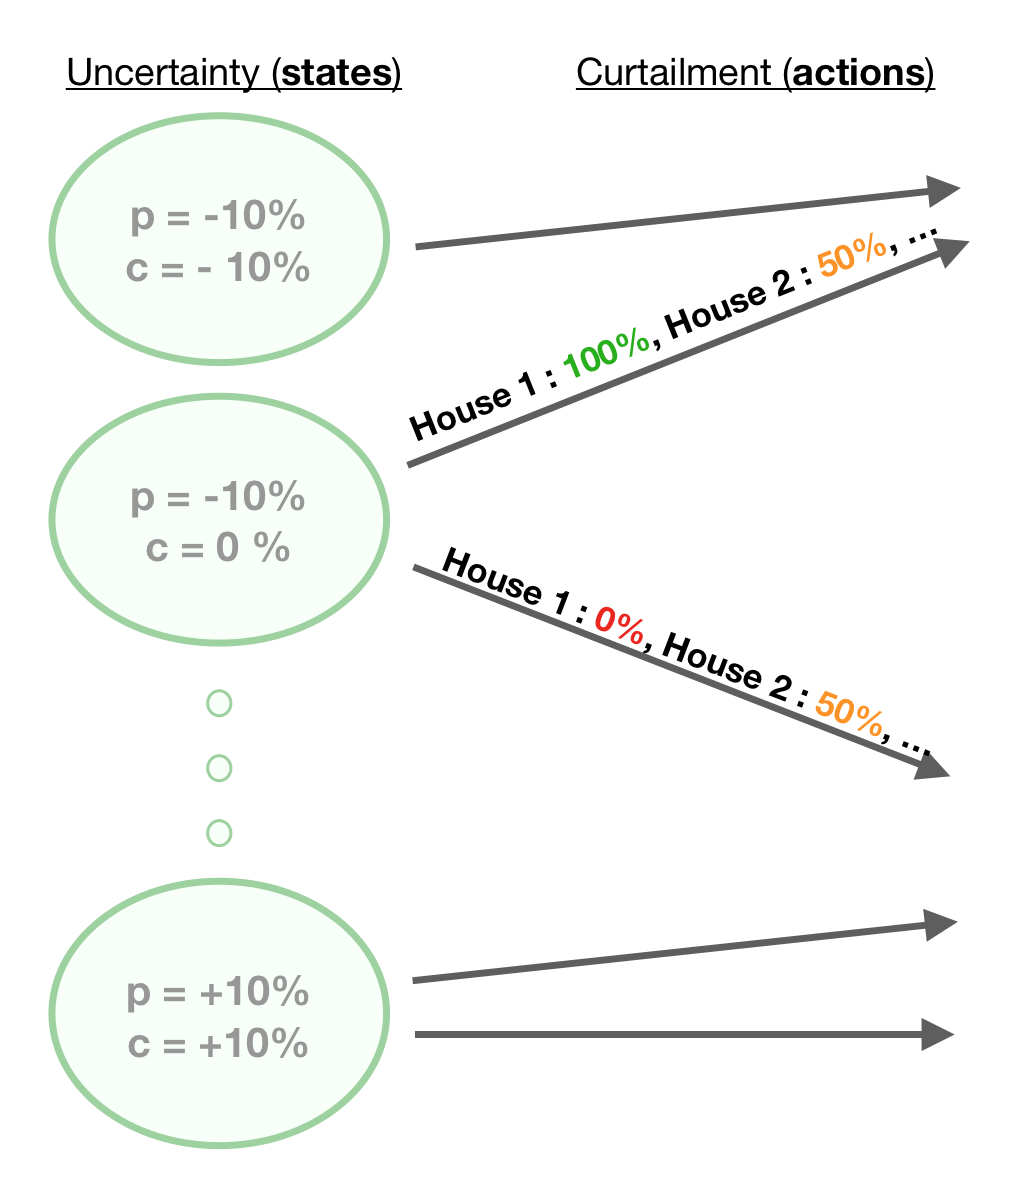
\includegraphics[scale=0.43]{./img/model_diagram.png}
  \end{center}
  \caption{Schematic representation of the states and control actions.}
  \label{fig:model_diag}
\end{figure}
